% Editable README diagram. The companion SVG uses the same geometry.
\documentclass[tikz,border=0pt]{standalone}
\usepackage[T1]{fontenc}
\usepackage{tgheros}
\renewcommand{\familydefault}{\sfdefault}
\usetikzlibrary{arrows.meta}
% Self-contained emoji-style vector fallback for minimal TeX installations.
\tikzset{
 pics/1f916/.style={code={
 \fill[gray!50,rounded corners=4pt] (2,5) rectangle (38,32);
 \draw[gray,line width=2pt] (20,32)--(20,38);\fill[red!70] (20,38) circle (3);
 \fill[cyan!25] (5,10) rectangle (35,29);
 \fill[white] (11,23) circle (4);\fill[white] (29,23) circle (4);
 \fill[black!70] (11,23) circle (2);\fill[black!70] (29,23) circle (2);
 \draw[black!60,line width=2pt] (12,14)--(28,14);
 \fill[red!65] (0,14) rectangle (3,25);\fill[red!65] (37,14) rectangle (40,25);
 }},
 pics/1f4c4/.style={code={
 \fill[white,draw=gray!45] (5,1)--(34,1)--(34,29)--(25,38)--(5,38)--cycle;
 \fill[blue!20] (25,38)--(25,29)--(34,29)--cycle;
 \foreach \y in {9,15,21}{\draw[blue!40,line width=1.4pt] (11,\y)--(28,\y);}
 }},
 pics/1f4da/.style={code={
 \foreach \y/\c in {3/blue,14/green,25/red}{
 \fill[\c!65,rounded corners=1pt] (3,\y) rectangle (37,\y+10);
 \fill[white!90!gray] (8,\y+2) rectangle (36,\y+7);}
 }},
 pics/270f/.style={code={
 \begin{scope}[rotate around={-38:(20,20)}]
 \fill[yellow!75!orange] (15,9) rectangle (25,33);
 \fill[pink] (15,33) rectangle (25,39);
 \fill[brown!35] (15,9)--(25,9)--(20,1)--cycle;
 \fill[black!70] (18,4)--(22,4)--(20,1)--cycle;
 \end{scope}
 }},
 pics/1f4bb/.style={code={
 \fill[gray!65,rounded corners=2pt] (4,11) rectangle (36,36);
 \fill[cyan!25] (7,14) rectangle (33,33);
 \fill[gray!40] (4,11)--(36,11)--(40,3)--(0,3)--cycle;
 \draw[white,line width=1.3pt] (11,25)--(16,21)--(11,17);
 }},
 pics/1f4ad/.style={code={
 \fill[white,draw=gray!40] (21,23) ellipse (18 and 13);
 \fill[white,draw=gray!40] (8,7) circle (4);
 \fill[white,draw=gray!40] (2,1) circle (2);
 }},
 pics/1f9e0/.style={code={
 \fill[pink!80] (12,20) ellipse (11 and 16);
 \fill[pink!80] (28,20) ellipse (11 and 16);
 \draw[red!40,line width=1.4pt] (20,7)--(20,33);
 \draw[red!40,line width=1.4pt] (9,29)--(14,25)--(9,19)--(14,14);
 \draw[red!40,line width=1.4pt] (31,29)--(26,25)--(31,19)--(26,14);
 }},
 pics/1f513/.style={code={
 \draw[gray!70,line width=4pt,rounded corners=6pt] (11,23)--(11,37)--(29,37)--(29,31);
 \fill[yellow!75!orange,rounded corners=3pt] (5,2) rectangle (35,25);
 \fill[brown!70] (20,16) circle (3);\draw[brown!70,line width=2pt] (20,15)--(20,9);
 }},
 pics/2705/.style={code={
 \fill[green!55!black,rounded corners=4pt] (2,2) rectangle (38,38);
 \draw[white,line width=4pt,line cap=round,line join=round] (9,21)--(17,12)--(31,29);
 }}
}
\newcommand{\jetemoji}[2]{\tikz[x=#1/40,y=#1/40]{\pic {#2};}}
\definecolor{color0}{HTML}{f5f8fc}
\definecolor{color1}{HTML}{20364f}
\definecolor{color2}{HTML}{65778c}
\definecolor{color3}{HTML}{ffffff}
\definecolor{color4}{HTML}{bfd8e7}
\definecolor{color5}{HTML}{167b9d}
\definecolor{color6}{HTML}{edf5fb}
\definecolor{color7}{HTML}{edf2f8}
\definecolor{color8}{HTML}{dce4ed}
\definecolor{color9}{HTML}{8559bb}
\definecolor{color10}{HTML}{d9c9eb}
\definecolor{color11}{HTML}{e9edf4}
\definecolor{color12}{HTML}{c7d0db}
\definecolor{color13}{HTML}{eaf6f0}
\definecolor{color14}{HTML}{b5dac9}
\definecolor{color15}{HTML}{168369}
\definecolor{color16}{HTML}{f1ecf8}
\begin{document}
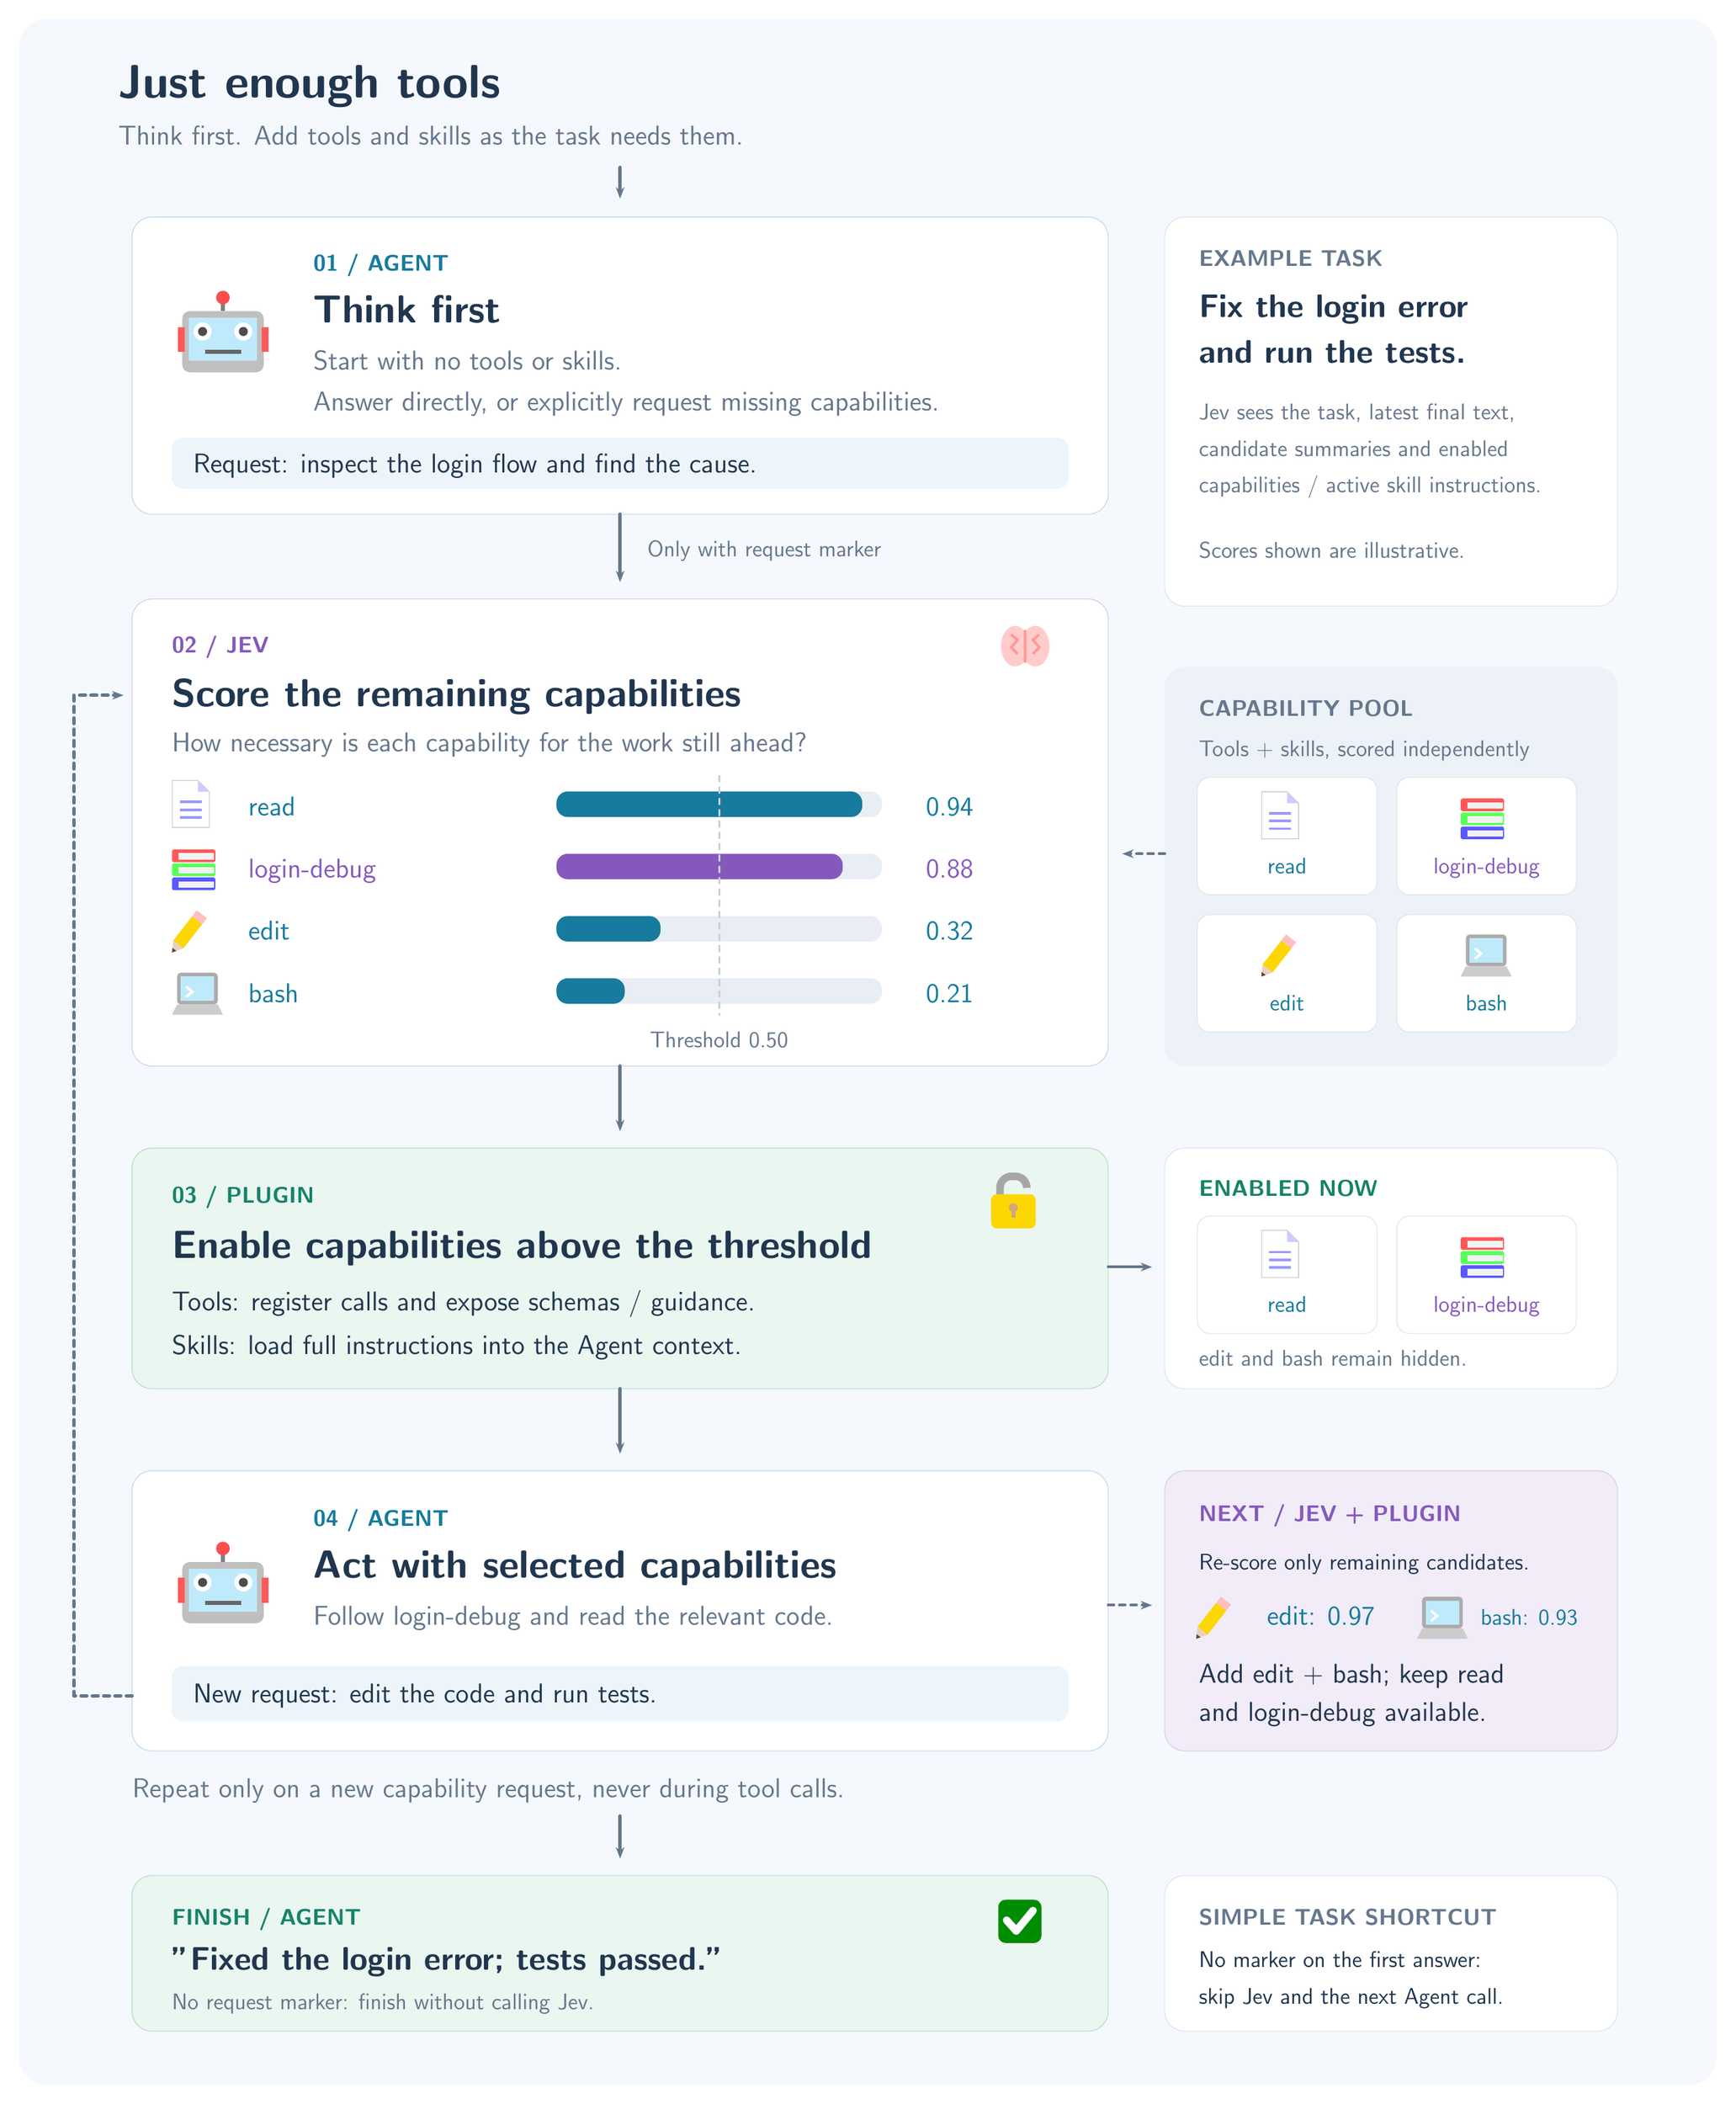
\begin{tikzpicture}[x=0.75pt,y=-0.75pt]
\path[fill=color0,draw=none,rounded corners=15.0pt] (0,0) rectangle (1200,1460);
\node[anchor=base west,inner sep=0pt,text=color1,font={\sffamily\fontsize{25.5}{30.6}\selectfont\bfseries}] at (70,56) {Just enough tools};
\node[anchor=base west,inner sep=0pt,text=color2,font={\sffamily\fontsize{15.0}{18.0}\selectfont}] at (70,89) {Think first. Add tools and skills as the task needs them.};
\draw[draw=color2,line width=1.875pt,line cap=round,line join=round,-{Stealth[length=6pt]}] (425,105) -- (425,127);
\path[fill=color3,draw=color4,rounded corners=10.5pt] (80,140) rectangle (770,350);
\node[anchor=south west,inner sep=0pt] at (112,250) {\jetemoji{48.0pt}{1f916}};
\node[anchor=base west,inner sep=0pt,text=color5,font={\sffamily\fontsize{12.0}{14.4}\selectfont\bfseries}] at (208,178) {01 / AGENT};
\node[anchor=base west,inner sep=0pt,text=color1,font={\sffamily\fontsize{21.0}{25.2}\selectfont\bfseries}] at (208,215) {Think first};
\node[anchor=base west,inner sep=0pt,text=color2,font={\sffamily\fontsize{15.0}{18.0}\selectfont}] at (208,248) {Start with no tools or skills.};
\node[anchor=base west,inner sep=0pt,text=color2,font={\sffamily\fontsize{13.5}{16.2}\selectfont}] at (208,277) {Answer directly, or explicitly request missing capabilities.};
\path[fill=color6,draw=none,rounded corners=6.0pt] (108,296) rectangle (742,332);
\node[anchor=base west,inner sep=0pt,text=color1,font={\sffamily\fontsize{13.5}{16.2}\selectfont}] at (123,321) {Request: inspect the login flow and find the cause.};
\path[fill=color7,draw=none,rounded corners=10.5pt] (810,458) rectangle (1130,740);
\node[anchor=base west,inner sep=0pt,text=color2,font={\sffamily\fontsize{12.0}{14.4}\selectfont\bfseries}] at (834,493) {CAPABILITY POOL};
\node[anchor=base west,inner sep=0pt,text=color2,font={\sffamily\fontsize{12.75}{15.3}\selectfont}] at (834,521) {Tools + skills, scored independently};
\path[fill=color3,draw=color8,rounded corners=6.75pt] (833,536) rectangle (960,619);
\node[anchor=south west,inner sep=0pt] at (878,580) {\jetemoji{27.0pt}{1f4c4}};
\node[anchor=base,inner sep=0pt,text=color5,font={\sffamily\fontsize{12.0}{14.4}\selectfont}] at (896.5,604) {read};
\path[fill=color3,draw=color8,rounded corners=6.75pt] (974,536) rectangle (1101,619);
\node[anchor=south west,inner sep=0pt] at (1019,580) {\jetemoji{27.0pt}{1f4da}};
\node[anchor=base,inner sep=0pt,text=color9,font={\sffamily\fontsize{12.0}{14.4}\selectfont}] at (1037.5,604) {login-debug};
\path[fill=color3,draw=color8,rounded corners=6.75pt] (833,633) rectangle (960,716);
\node[anchor=south west,inner sep=0pt] at (878,677) {\jetemoji{27.0pt}{270f}};
\node[anchor=base,inner sep=0pt,text=color5,font={\sffamily\fontsize{12.0}{14.4}\selectfont}] at (896.5,701) {edit};
\path[fill=color3,draw=color8,rounded corners=6.75pt] (974,633) rectangle (1101,716);
\node[anchor=south west,inner sep=0pt] at (1019,677) {\jetemoji{27.0pt}{1f4bb}};
\node[anchor=base,inner sep=0pt,text=color5,font={\sffamily\fontsize{12.0}{14.4}\selectfont}] at (1037.5,701) {bash};
\draw[draw=color2,line width=1.875pt,line cap=round,line join=round,-{Stealth[length=6pt]}] (425,350) -- (425,398);
\node[anchor=base west,inner sep=0pt,text=color2,font={\sffamily\fontsize{12.75}{15.3}\selectfont}] at (444,380) {Only with request marker};
\path[fill=color3,draw=color10,rounded corners=10.5pt] (80,410) rectangle (770,740);
\node[anchor=base west,inner sep=0pt,text=color9,font={\sffamily\fontsize{12.0}{14.4}\selectfont\bfseries}] at (108,448) {02 / JEV};
\node[anchor=south west,inner sep=0pt] at (694,458) {\jetemoji{27.0pt}{1f9e0}};
\node[anchor=base west,inner sep=0pt,text=color1,font={\sffamily\fontsize{20.25}{24.3}\selectfont\bfseries}] at (108,486) {Score the remaining capabilities};
\node[anchor=base west,inner sep=0pt,text=color2,font={\sffamily\fontsize{13.5}{16.2}\selectfont}] at (108,518) {How necessary is each capability for the work still ahead?};
\node[anchor=south west,inner sep=0pt] at (108,572) {\jetemoji{27.0pt}{1f4c4}};
\node[anchor=base west,inner sep=0pt,text=color5,font={\sffamily\fontsize{14.25}{17.1}\selectfont}] at (162,563) {read};
\path[fill=color11,draw=none,rounded corners=6.0pt] (380,546) rectangle (610,564);
\path[fill=color5,draw=none,rounded corners=6.0pt] (380,546) rectangle (596.2,564);
\node[anchor=base west,inner sep=0pt,text=color5,font={\sffamily\fontsize{14.25}{17.1}\selectfont}] at (641,563) {0.94};
\node[anchor=south west,inner sep=0pt] at (108,616) {\jetemoji{27.0pt}{1f4da}};
\node[anchor=base west,inner sep=0pt,text=color9,font={\sffamily\fontsize{14.25}{17.1}\selectfont}] at (162,607) {login-debug};
\path[fill=color11,draw=none,rounded corners=6.0pt] (380,590) rectangle (610,608);
\path[fill=color9,draw=none,rounded corners=6.0pt] (380,590) rectangle (582.4,608);
\node[anchor=base west,inner sep=0pt,text=color9,font={\sffamily\fontsize{14.25}{17.1}\selectfont}] at (641,607) {0.88};
\node[anchor=south west,inner sep=0pt] at (108,660) {\jetemoji{27.0pt}{270f}};
\node[anchor=base west,inner sep=0pt,text=color5,font={\sffamily\fontsize{14.25}{17.1}\selectfont}] at (162,651) {edit};
\path[fill=color11,draw=none,rounded corners=6.0pt] (380,634) rectangle (610,652);
\path[fill=color5,draw=none,rounded corners=6.0pt] (380,634) rectangle (453.6,652);
\node[anchor=base west,inner sep=0pt,text=color5,font={\sffamily\fontsize{14.25}{17.1}\selectfont}] at (641,651) {0.32};
\node[anchor=south west,inner sep=0pt] at (108,704) {\jetemoji{27.0pt}{1f4bb}};
\node[anchor=base west,inner sep=0pt,text=color5,font={\sffamily\fontsize{14.25}{17.1}\selectfont}] at (162,695) {bash};
\path[fill=color11,draw=none,rounded corners=6.0pt] (380,678) rectangle (610,696);
\path[fill=color5,draw=none,rounded corners=6.0pt] (380,678) rectangle (428.3,696);
\node[anchor=base west,inner sep=0pt,text=color5,font={\sffamily\fontsize{14.25}{17.1}\selectfont}] at (641,695) {0.21};
\draw[draw=color12,line width=1.125pt,line cap=round,line join=round,dashed] (495,535) -- (495,704);
\node[anchor=base,inner sep=0pt,text=color2,font={\sffamily\fontsize{12.0}{14.4}\selectfont}] at (495,727) {Threshold 0.50};
\draw[draw=color2,line width=1.5pt,line cap=round,line join=round,-{Stealth[length=6pt]},dashed] (810,590) -- (780,590);
\path[fill=color3,draw=color8,rounded corners=10.5pt] (810,140) rectangle (1130,415);
\node[anchor=base west,inner sep=0pt,text=color2,font={\sffamily\fontsize{12.0}{14.4}\selectfont\bfseries}] at (834,175) {EXAMPLE TASK};
\node[anchor=base west,inner sep=0pt,text=color1,font={\sffamily\fontsize{18.0}{21.6}\selectfont\bfseries}] at (834,211) {Fix the login error};
\node[anchor=base west,inner sep=0pt,text=color1,font={\sffamily\fontsize{18.0}{21.6}\selectfont\bfseries}] at (834,243) {and run the tests.};
\node[anchor=base west,inner sep=0pt,text=color2,font={\sffamily\fontsize{12.75}{15.3}\selectfont}] at (834,283) {Jev sees the task, latest final text,};
\node[anchor=base west,inner sep=0pt,text=color2,font={\sffamily\fontsize{12.75}{15.3}\selectfont}] at (834,309) {candidate summaries and enabled};
\node[anchor=base west,inner sep=0pt,text=color2,font={\sffamily\fontsize{12.75}{15.3}\selectfont}] at (834,335) {capabilities / active skill instructions.};
\node[anchor=base west,inner sep=0pt,text=color2,font={\sffamily\fontsize{12.0}{14.4}\selectfont}] at (834,381) {Scores shown are illustrative.};
\draw[draw=color2,line width=1.875pt,line cap=round,line join=round,-{Stealth[length=6pt]}] (425,740) -- (425,786);
\path[fill=color13,draw=color14,rounded corners=10.5pt] (80,798) rectangle (770,968);
\node[anchor=base west,inner sep=0pt,text=color15,font={\sffamily\fontsize{12.0}{14.4}\selectfont\bfseries}] at (108,837) {03 / PLUGIN};
\node[anchor=south west,inner sep=0pt] at (687,855) {\jetemoji{31.5pt}{1f513}};
\node[anchor=base west,inner sep=0pt,text=color1,font={\sffamily\fontsize{19.5}{23.400000000000002}\selectfont\bfseries}] at (108,876) {Enable capabilities above the threshold};
\node[anchor=base west,inner sep=0pt,text=color1,font={\sffamily\fontsize{14.25}{17.1}\selectfont}] at (108,913) {Tools: register calls and expose schemas / guidance.};
\node[anchor=base west,inner sep=0pt,text=color1,font={\sffamily\fontsize{14.25}{17.1}\selectfont}] at (108,944) {Skills: load full instructions into the Agent context.};
\path[fill=color3,draw=color8,rounded corners=10.5pt] (810,798) rectangle (1130,968);
\node[anchor=base west,inner sep=0pt,text=color15,font={\sffamily\fontsize{12.0}{14.4}\selectfont\bfseries}] at (834,832) {ENABLED NOW};
\path[fill=color3,draw=color8,rounded corners=6.75pt] (833,846) rectangle (960,929);
\node[anchor=south west,inner sep=0pt] at (878,890) {\jetemoji{27.0pt}{1f4c4}};
\node[anchor=base,inner sep=0pt,text=color5,font={\sffamily\fontsize{12.0}{14.4}\selectfont}] at (896.5,914) {read};
\path[fill=color3,draw=color8,rounded corners=6.75pt] (974,846) rectangle (1101,929);
\node[anchor=south west,inner sep=0pt] at (1019,890) {\jetemoji{27.0pt}{1f4da}};
\node[anchor=base,inner sep=0pt,text=color9,font={\sffamily\fontsize{12.0}{14.4}\selectfont}] at (1037.5,914) {login-debug};
\node[anchor=base west,inner sep=0pt,text=color2,font={\sffamily\fontsize{12.75}{15.3}\selectfont}] at (834,952) {edit and bash remain hidden.};
\draw[draw=color2,line width=1.5pt,line cap=round,line join=round,-{Stealth[length=6pt]}] (770,882) -- (801,882);
\draw[draw=color2,line width=1.875pt,line cap=round,line join=round,-{Stealth[length=6pt]}] (425,968) -- (425,1014);
\path[fill=color3,draw=color4,rounded corners=10.5pt] (80,1026) rectangle (770,1224);
\node[anchor=south west,inner sep=0pt] at (112,1134) {\jetemoji{48.0pt}{1f916}};
\node[anchor=base west,inner sep=0pt,text=color5,font={\sffamily\fontsize{12.0}{14.4}\selectfont\bfseries}] at (208,1065) {04 / AGENT};
\node[anchor=base west,inner sep=0pt,text=color1,font={\sffamily\fontsize{19.5}{23.400000000000002}\selectfont\bfseries}] at (208,1102) {Act with selected capabilities};
\node[anchor=base west,inner sep=0pt,text=color2,font={\sffamily\fontsize{13.5}{16.2}\selectfont}] at (208,1135) {Follow login-debug and read the relevant code.};
\path[fill=color6,draw=none,rounded corners=6.0pt] (108,1164) rectangle (742,1203);
\node[anchor=base west,inner sep=0pt,text=color1,font={\sffamily\fontsize{13.5}{16.2}\selectfont}] at (123,1190) {New request: edit the code and run tests.};
\path[fill=color16,draw=color10,rounded corners=10.5pt] (810,1026) rectangle (1130,1224);
\node[anchor=base west,inner sep=0pt,text=color9,font={\sffamily\fontsize{12.0}{14.4}\selectfont\bfseries}] at (834,1062) {NEXT / JEV + PLUGIN};
\node[anchor=base west,inner sep=0pt,text=color1,font={\sffamily\fontsize{12.75}{15.3}\selectfont}] at (834,1096) {Re-score only remaining candidates.};
\node[anchor=south west,inner sep=0pt] at (832,1145) {\jetemoji{27.0pt}{270f}};
\node[anchor=base west,inner sep=0pt,text=color5,font={\sffamily\fontsize{13.5}{16.2}\selectfont}] at (882,1135) {edit: 0.97};
\node[anchor=south west,inner sep=0pt] at (988,1145) {\jetemoji{27.0pt}{1f4bb}};
\node[anchor=base west,inner sep=0pt,text=color5,font={\sffamily\fontsize{12.0}{14.4}\selectfont}] at (1033,1135) {bash: 0.93};
\node[anchor=base west,inner sep=0pt,text=color1,font={\sffamily\fontsize{13.5}{16.2}\selectfont}] at (834,1176) {Add edit + bash; keep read};
\node[anchor=base west,inner sep=0pt,text=color1,font={\sffamily\fontsize{13.5}{16.2}\selectfont}] at (834,1203) {and login-debug available.};
\draw[draw=color2,line width=1.5pt,line cap=round,line join=round,-{Stealth[length=6pt]},dashed] (770,1121) -- (801,1121);
\draw[draw=color2,line width=1.875pt,line cap=round,line join=round,-{Stealth[length=6pt]},dashed] (80,1185) -- (39,1185) -- (39,478) -- (74,478);
\node[anchor=base west,inner sep=0pt,text=color2,font={\sffamily\fontsize{13.5}{16.2}\selectfont}] at (80,1257) {Repeat only on a new capability request, never during tool calls.};
\draw[draw=color2,line width=1.875pt,line cap=round,line join=round,-{Stealth[length=6pt]}] (425,1270) -- (425,1300);
\path[fill=color13,draw=color14,rounded corners=10.5pt] (80,1312) rectangle (770,1422);
\node[anchor=base west,inner sep=0pt,text=color15,font={\sffamily\fontsize{12.0}{14.4}\selectfont\bfseries}] at (108,1347) {FINISH / AGENT};
\node[anchor=south west,inner sep=0pt] at (692,1360) {\jetemoji{25.5pt}{2705}};
\node[anchor=base west,inner sep=0pt,text=color1,font={\sffamily\fontsize{17.25}{20.7}\selectfont\bfseries}] at (108,1379) {"Fixed the login error; tests passed."};
\node[anchor=base west,inner sep=0pt,text=color2,font={\sffamily\fontsize{12.75}{15.3}\selectfont}] at (108,1407) {No request marker: finish without calling Jev.};
\path[fill=color3,draw=color8,rounded corners=10.5pt] (810,1312) rectangle (1130,1422);
\node[anchor=base west,inner sep=0pt,text=color2,font={\sffamily\fontsize{12.0}{14.4}\selectfont\bfseries}] at (834,1347) {SIMPLE TASK SHORTCUT};
\node[anchor=base west,inner sep=0pt,text=color1,font={\sffamily\fontsize{12.75}{15.3}\selectfont}] at (834,1377) {No marker on the first answer:};
\node[anchor=base west,inner sep=0pt,text=color1,font={\sffamily\fontsize{12.75}{15.3}\selectfont}] at (834,1403) {skip Jev and the next Agent call.};
\end{tikzpicture}
\end{document}
